\subsection{El Fibrado Tangente}\label{Subsección: Fibrado Tangente}
Por la definición que hemos dado de espacio tangente, estos están definidos en cada punto de una variedad suave, sin embargo, para algunos fines es más conveniente considerar todos los espacios tangentes a una variedad de forma simultánea. Es con este propósito que definiremos al Fibrado Tangente de una variedad suave, este objeto nos dará una manera de organizar los espacios tangentes de una variedad suave de tal modo que el objeto resultante sea en sí mismo una variedad suave.

\begin{center}
	\begin{figure}[h!]
		\centering
		\begin{subfigure}{0.35\textwidth}
			\centering
			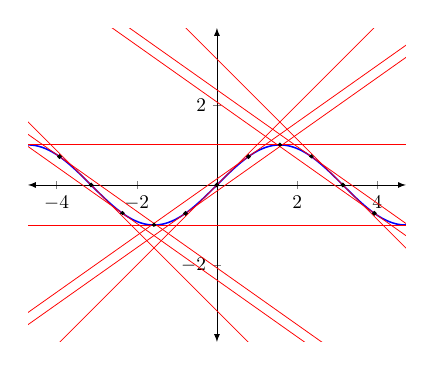
\begin{tikzpicture}[scale=0.70]
	\begin{axis}[
			% grid=both,
			xmin=-3*pi/2,
			xmax=3*pi/2,
			ymin=-1.6,
			ymax=1.6,
			axis lines=middle,
			axis line style={latex-latex},
			axis equal,
		]

		\addplot[
			samples=200,
			domain=-4*pi:4*pi,
			color=blue,
			thick,
			smooth,
		]
		{sin(deg(x))};
\addplot[domain=-5:5,color=red,thin]{-0.707107 * (x + 3.926991) + 0.707107};
\addplot+[mark=*, mark options={black},mark size=1pt] coordinates {( -3.926991 , 0.707107 )};
\addplot[domain=-5:5,color=red,thin]{-1.000000 * (x + 3.141593) + -0.000000};
\addplot+[mark=*, mark options={black},mark size=1pt] coordinates {( -3.141593 , -0.000000 )};
\addplot[domain=-5:5,color=red,thin]{-0.707107 * (x + 2.356194) + -0.707107};
\addplot+[mark=*, mark options={black},mark size=1pt] coordinates {( -2.356194 , -0.707107 )};
\addplot[domain=-5:5,color=red,thin]{0.000000 * (x + 1.570796) + -1.000000};
\addplot+[mark=*, mark options={black},mark size=1pt] coordinates {( -1.570796 , -1.000000 )};
\addplot[domain=-5:5,color=red,thin]{0.707107 * (x + 0.785398) + -0.707107};
\addplot+[mark=*, mark options={black},mark size=1pt] coordinates {( -0.785398 , -0.707107 )};
\addplot[domain=-5:5,color=red,thin]{1.000000 * (x - 0.000000) - -0.000000};
\addplot+[mark=*, mark options={black},mark size=1pt] coordinates {( 0.000000 , 0.000000 )};
\addplot[domain=-5:5,color=red,thin]{0.707107 * (x - 0.785398) - -0.707107};
\addplot+[mark=*, mark options={black},mark size=1pt] coordinates {( 0.785398 , 0.707107 )};
\addplot[domain=-5:5,color=red,thin]{-0.000000 * (x - 1.570796) - -1.000000};
\addplot+[mark=*, mark options={black},mark size=1pt] coordinates {( 1.570796 , 1.000000 )};
\addplot[domain=-5:5,color=red,thin]{-0.707107 * (x - 2.356195) - -0.707107};
\addplot+[mark=*, mark options={black},mark size=1pt] coordinates {( 2.356195 , 0.707107 )};
\addplot[domain=-5:5,color=red,thin]{-1.000000 * (x - 3.141593) - 0.000000};
\addplot+[mark=*, mark options={black},mark size=1pt] coordinates {( 3.141593 , -0.000000 )};
\addplot[domain=-5:5,color=red,thin]{-0.707107 * (x - 3.926991) - 0.707107};
\addplot+[mark=*, mark options={black},mark size=1pt] coordinates {( 3.926991 , -0.707107 )};	\end{axis}
\end{tikzpicture}

		\end{subfigure}
		\hspace{40pt}
		\begin{subfigure}{0.35\textwidth}
			\centering
			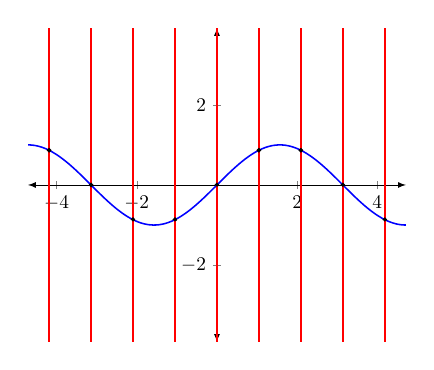
\begin{tikzpicture}[scale=0.70]
	\begin{axis}[
			% grid=both,
			xmin=-3*pi/2,
			xmax=3*pi/2,
			ymin=-1.6,
			ymax=1.6,
			axis lines=middle,
			axis line style={latex-latex},
			axis equal,
		]

		\addplot[
			samples=200,
			domain=-4*pi:4*pi,
			color=blue,
			thick,
			smooth,
		]
		{sin(deg(x))};

\addplot+[mark=*, mark options={black},mark size=1pt] coordinates {( -4.188790 , 0.866025 )};
\addplot[thick, smooth,domain=-pi:pi,red] coordinates {(-4.188790,-5)(-4.188790,5)};
\addplot+[mark=*, mark options={black},mark size=1pt] coordinates {( -3.141593 , -0.000000 )};
\addplot[thick, smooth,domain=-pi:pi,red] coordinates {(-3.141593,-5)(-3.141593,5)};
\addplot+[mark=*, mark options={black},mark size=1pt] coordinates {( -2.094395 , -0.866025 )};
\addplot[thick, smooth,domain=-pi:pi,red] coordinates {(-2.094395,-5)(-2.094395,5)};
\addplot+[mark=*, mark options={black},mark size=1pt] coordinates {( -1.047197 , -0.866025 )};
\addplot[thick, smooth,domain=-pi:pi,red] coordinates {(-1.047197,-5)(-1.047197,5)};
\addplot+[mark=*, mark options={black},mark size=1pt] coordinates {( 0.000000 , 0.000000 )};
\addplot[thick, smooth,domain=-pi:pi,red] coordinates {(0.000000,-5)(0.000000,5)};
\addplot+[mark=*, mark options={black},mark size=1pt] coordinates {( 1.047198 , 0.866025 )};
\addplot[thick, smooth,domain=-pi:pi,red] coordinates {(1.047198,-5)(1.047198,5)};
\addplot+[mark=*, mark options={black},mark size=1pt] coordinates {( 2.094395 , 0.866025 )};
\addplot[thick, smooth,domain=-pi:pi,red] coordinates {(2.094395,-5)(2.094395,5)};
\addplot+[mark=*, mark options={black},mark size=1pt] coordinates {( 3.141593 , -0.000000 )};
\addplot[thick, smooth,domain=-pi:pi,red] coordinates {(3.141593,-5)(3.141593,5)};
\addplot+[mark=*, mark options={black},mark size=1pt] coordinates {( 4.188790 , -0.866026 )};
\addplot[thick, smooth,domain=-pi:pi,red] coordinates {(4.188790,-5)(4.188790,5)};	

\end{axis}
\end{tikzpicture}

		\end{subfigure}
		\\[20pt]
		\begin{subfigure}{0.35\textwidth}
			\centering
			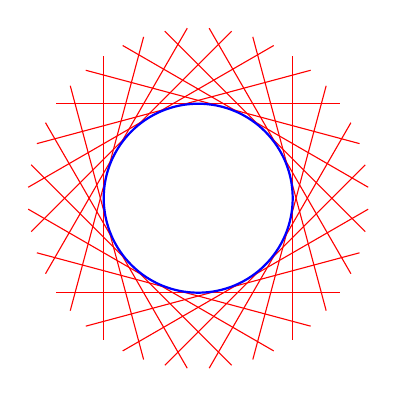
\begin{tikzpicture}[scale=1.20]
  % Lineas iniciales
  \draw[red] (-1,-1.5) -- (-1,1.5);
  \draw[red] (1,-1.5)  -- (1,1.5);
  \draw[red] (-1.5,1)  -- (1.5,1);
	\draw[red] (-1.5,-1) -- (1.5,-1);

	\begin{scope}[rotate around={15:(0,0)}]
		\draw[red] (-1,-1.5) -- (-1,1.5);
		\draw[red] (1,-1.5)  -- (1,1.5);
		\draw[red] (-1.5,1)  -- (1.5,1);
		\draw[red] (-1.5,-1) -- (1.5,-1);
	\end{scope}
	\begin{scope}[rotate around={30:(0,0)}]
		\draw[red] (-1,-1.5) -- (-1,1.5);
		\draw[red] (1,-1.5)  -- (1,1.5);
		\draw[red] (-1.5,1)  -- (1.5,1);
		\draw[red] (-1.5,-1) -- (1.5,-1);
	\end{scope}
	\begin{scope}[rotate around={45:(0,0)}]
		\draw[red] (-1,-1.5) -- (-1,1.5);
		\draw[red] (1,-1.5)  -- (1,1.5);
		\draw[red] (-1.5,1)  -- (1.5,1);
		\draw[red] (-1.5,-1) -- (1.5,-1);
	\end{scope}
	\begin{scope}[rotate around={60:(0,0)}]
		\draw[red] (-1,-1.5) -- (-1,1.5);
		\draw[red] (1,-1.5)  -- (1,1.5);
		\draw[red] (-1.5,1)  -- (1.5,1);
		\draw[red] (-1.5,-1) -- (1.5,-1);
	\end{scope}
	\begin{scope}[rotate around={75:(0,0)}]
		\draw[red] (-1,-1.5) -- (-1,1.5);
		\draw[red] (1,-1.5)  -- (1,1.5);
		\draw[red] (-1.5,1)  -- (1.5,1);
		\draw[red] (-1.5,-1) -- (1.5,-1);
	\end{scope}

	\draw[blue,thick] (0,0) circle (1);
\end{tikzpicture}

		\end{subfigure}
		\hspace{30pt}
		\begin{subfigure}{0.35\textwidth}
			\centering
			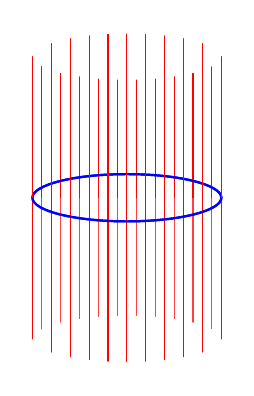
\begin{tikzpicture}[scale=1.20]
  \path[use as bounding box] (-1.05,-1.8) rectangle (1.05,1.8);

	% Lineas Traseras
	\draw[color=red,opacity=0.75] (0.1,-2.0) -- (0.1,0.0);
	\draw[color=red,opacity=0.75] (0.3,-2.0) -- (0.3,0.0);
	\draw[color=red,opacity=0.75] (0.5,-2.0) -- (0.5,0.0);
	\draw[color=red,opacity=0.75] (0.7,-2.0) -- (0.7,0.0);
	\draw[color=red,opacity=0.75] (0.9,-2.0) -- (0.9,0.0);
	\draw[color=red,opacity=0.75] (-0.1,-2.0) -- (-0.1,0.0);
	\draw[color=red,opacity=0.75] (-0.3,-2.0) -- (-0.3,0.0);
	\draw[color=red,opacity=0.75] (-0.5,-2.0) -- (-0.5,0.0);
	\draw[color=red,opacity=0.75] (-0.7,-2.0) -- (-0.7,0.0);
	\draw[color=red,opacity=0.75] (-0.9,-2.0) -- (-0.9,0.0);
	\fill[white] (-1,-1.5) arc (0:180:-1 and 0.25) -- (1,-2) -- (-1,-2)--(-1,-1.5);

	% Elipse
	\draw[blue,thick] (0,0) ellipse (1 and 0.25);

	% Lineas Frontales
	\draw[red] (0.0,-2.0) -- (0.0,0.0);
	\draw[red] (0.2,-2.0) -- (0.2,0.0);
	\draw[red] (0.4,-2.0) -- (0.4,0.0);
	\draw[red] (0.6,-2.0) -- (0.6,0.0);
	\draw[red] (0.8,-2.0) -- (0.8,0.0);
	\draw[red] (1.0,-2.0) -- (1.0,0.0);
	\draw[red] (-0.2,-2.0) -- (-0.2,0.0);
	\draw[red] (-0.4,-2.0) -- (-0.4,0.0);
	\draw[red] (-0.6,-2.0) -- (-0.6,0.0);
	\draw[red] (-0.8,-2.0) -- (-0.8,0.0);
	\draw[red] (-1.0,-2.0) -- (-1.0,0.0);

  \draw[thick,white,fill=white] (-1,-1.50) arc (0:180:-1 and -0.25) -- (1,-2) -- (-1,-2) -- cycle;

	\begin{scope}[rotate around={180:(0,0)}]
	\draw[red] (0.1,-2.0) -- (0.1,0.0);
	\draw[red] (0.3,-2.0) -- (0.3,0.0);
	\draw[red] (0.5,-2.0) -- (0.5,0.0);
	\draw[red] (0.7,-2.0) -- (0.7,0.0);
	\draw[red] (0.9,-2.0) -- (0.9,0.0);
	\draw[red] (-0.1,-2.0) -- (-0.1,0.0);
	\draw[red] (-0.3,-2.0) -- (-0.3,0.0);
	\draw[red] (-0.5,-2.0) -- (-0.5,0.0);
	\draw[red] (-0.7,-2.0) -- (-0.7,0.0);
	\draw[red] (-0.9,-2.0) -- (-0.9,0.0);
	\fill[white] (-1,-1.5) arc (0:180:-1 and 0.25) -- (1,-2) -- (-1,-2)--(-1,-1.5);

	% Elipse
	\draw[blue,thick] (0,0) ellipse (1 and 0.25);

	% Lineas Frontales
	\draw[red] (0.0,-2.0) -- (0.0,0.0);
	\draw[red] (0.2,-2.0) -- (0.2,0.0);
	\draw[red] (0.4,-2.0) -- (0.4,0.0);
	\draw[red] (0.6,-2.0) -- (0.6,0.0);
	\draw[red] (0.8,-2.0) -- (0.8,0.0);
	\draw[red] (1.0,-2.0) -- (1.0,0.0);
	\draw[red] (-0.2,-2.0) -- (-0.2,0.0);
	\draw[red] (-0.4,-2.0) -- (-0.4,0.0);
	\draw[red] (-0.6,-2.0) -- (-0.6,0.0);
	\draw[red] (-0.8,-2.0) -- (-0.8,0.0);
	\draw[red] (-1.0,-2.0) -- (-1.0,0.0);

	\draw[thick,white,fill=white] (-1,-1.5) arc (0:180:-1 and -0.25) -- (1,-2) -- (-1,-2) -- cycle;
	\end{scope}
\end{tikzpicture}

		\end{subfigure}
    \caption{Representación del fibrado tangente de dos variedades, $\sin(x)$ y $\S^{1}$.}
  \end{figure}
\end{center}

\begin{definition}[Fibrado Tangente]
	Dada una variedad suave $M$, definimos el \it{fibrado tangente de $M$} o \it{haz tangente de $M$}, el cual denotaremos por $TM$, como la unión disjunta de todos los espacios tangentes a $M$:
	\[ TM = \bigsqcup_{p \in M} T_p(M) = \bigcup_{p \in M} \{p\} \times T_p(M). \]
\end{definition}

Denotaremos a los elementos del conjunto como un par ordenado $(p, \omega)$, donde $p \in M$ y $\omega \in T_p(M)$. El fibrado tangente $TM$ tiene un mapa proyección natural sobre la variedad $M$, $\pi: TM \to M$ dado por $\pi(p,\omega)=p$.

\begin{theorem}\label{Teorema: Estructura de Variedad del Fibrado Tangente}
	Sea $M^n$ una variedad suave, el fibrado tangente $TM$ tiene una topología natural y una estructura suave que vuelven a $TM$ una variedad suave $2n-$dimensional de tal modo que la proyección $\pi: TM \to M$ es suave con respecto a dicha estructura suave.
\end{theorem}

\begin{proof}
	Para realizar esta demostración haremos uso del lema \ref{Lemma: Lema de Cartas Suaves de una Variedad}, mostraremos que $TM$ cumple las cinco propiedades ahí mencionadas cuando se da una colección adecuada de subconjuntos.

	Consideremos una carta suave $(U,\phi)=(U,\phi_1,\dots,\phi_n)$ de $M$, $\pi^{-1}(U) \subseteq TM$ será la colección formada por todos los vectores tangentes a $M$ en cada punto de $U$. Dado que cada $T_p(M)$ es un espacio vectorial y que, como hemos visto, $\{\left. \frac{\partial}{\partial \phi_{i}} \right|_{p}\}_{i=1}^{n}$ nos da una base para $T_p(M)$, cada vector tangente $\omega_p \in T_p(M)$ podrá ser escrito de forma única como una combinación lineal:
	\[
		\omega_p = \sum_{i=1}^{n} v_i \left. \frac{\partial}{\partial \phi_{i}}\right|_{p},
	\]
	donde cada $v_i$ es una constante que dependerá del vector tangente, $v_i = v_i(\omega_p) \in \R$. Definamos el mapa $\hat{\phi}: TM \to \R^{2n}$ como:
	\[
		\hat{\phi} \left(\sum_{i=1}^{n} v_i
		\left. \frac{\partial}{\partial \phi_{i}}\right|_{p} \right)
		=
		\left(\phi_1(p), \dots, \phi_n(p), v_1, \dots, v_n \right).
	\]
a
	Por cómo estamos definiendo este mapa, la imagen de $\pi^{-1}(U)$ bajo $\hat{\phi}$, $\hat{\phi}(\pi^{-1})(U)$ será el conjunto $\phi(U) \times \R^n$, que es un subconjunto abierto de $\R^{2n}$, y trivialmente será una biyección dado que el mapa inverso existe, de hecho, este puede ser escrito explícitamente como:
	\[
		\hat{\phi}^{-1}(\phi_{1},\dots, \phi_{n}, v_1, \dots, v_n)
		=
		\sum_{i=1}^{n} v_i \left. \frac{\partial}{\partial \phi_i} \right|_{\phi^{-1}(p)}.
	\]
	Por lo tanto, la condición 1 del lema se cumple.

	Para mostrar la segunda propiedad tomemos dos cartas suaves en $M$, $(U,\phi)$ y $(V,\psi)$, existirán cartas $(\pi^{-1}(U),\hat{\phi})$ y $(\pi^{-1}(V),\hat{\psi})$ en $TM$ correspondientes a las respectivas cartas en $M$. Notemos que, sin importar si la intersección es vacía se tiene que $\phi(U \cap V)$ y $\psi(U \cap V)$ son subconjuntos abiertos de $\R^n$, por lo que:
	\begin{align*}
		\hat{\phi}(\pi^{-1}(U) \cap \pi^{-1}(V)) & =
		\phi(U \cap V) \times \R^n,                  \\
		\hat{\psi}(\pi^{-1}(U) \cap \pi^{-1}(V)) & =
		\psi(U \cap V) \times \R^n.                  \\
	\end{align*}
	Son subconjuntos abiertos de $\R^{2n}$, esto implica que la propiedad 2 se cumple para estas cartas en $TM$.

	El mapa de transición $\hat{\psi} \circ \hat{\phi}^{-1}: \phi(U \cap V) \times \R^n \to \psi(U \cap V) \times \R^n$ puede ser expresado de manera explícita utilizando la identidad para el cambio de coordenadas mostrada en la sección anterior.
	\begin{align*}
		\hat{\psi} \circ \hat{\phi}^{-1}
		(\phi_1, \dots, \phi_n, v_1, \dots, v_n)
		 & =
		\hat{\psi} \left( \left.
		\sum_{i=1}^{n} v_i \frac{\partial}{\partial \phi_i}
		\right|_{\phi^{-1}(p)}\right)                      \\
		 & =
		\hat{\psi}\left(
		\sum_{i=1}^{n}
		\left(
		\sum_{j=1}^{n}
		\frac{\partial \psi_i}{\partial \phi_j} (\phi(p)) w_j
		\right)
		\left.
		\frac{\partial}{\partial \phi_i}
		\right|_{\phi^{-1}(p)}
		\right)
		\\
		 & =
		\Biggl(
		\psi_1(\phi^{-1}(p)), \dots, \psi_n(\phi^{-1}(p)), \\
		 & \quad \hspace{24pt}
		\sum_{j=1}^{n} \frac{\partial \psi_1}{\partial \phi_j}(\phi(p))w_j,
		\dots,
		\sum_{j=1}^{n} \frac{\partial \psi_n}{\partial \phi_j}(\phi(p))w_j
		\Biggr).
	\end{align*}
	Por lo tanto, cada una de las componentes es la composición de mapas suaves o la suma de mapas suaves, por lo que el mapa $\hat{\psi} \circ \phi^{-1}$ es suave, cumpliendo así la propiedad 3.

	Por la segundo numerabilidad de $M$ podemos elegir una colección numerable $\mathcal{U} = \{U_\alpha\}$ de cartas coordenadas, de la cual obtendremos la colección numerable $\{\pi^{-1}(U_\alpha)\}$ de cartas coordenadas que cubren a $TM$ y que como hemos visto cumplen las propiedades 1, 2 y 3, y la existencia de tal colección nos da la cuarta propiedad.

	Para la quinta y última propiedad notemos que si se damos dos elementos $(p,\omega)$ y $(q, \nu)$ de $TM$ entonces hay dos posibilidades, $p = q$, en cuyo caso habrá una vecindad $\pi^{-1}(U)$ que contiene a ambos o $p \neq q$, en cuyo caso existan vecindades disjuntas $U,V$ en $M$ tales que $p \in U$ y $q \in V$, de modo que $\pi^{-1}(U)$ y $\pi^{-1}(V)$ serán vecindades disjuntas de $(p,\omega)$ y $(q,\nu)$.

	Por lo tanto, podemos concluir que $TM$ es una variedad suave con la estructura suave dada por los conjuntos de la forma $\pi^{-1}(U)$. La suavidad de la proyección se garantiza por el teorema \ref{Teorema: Mapa a Producto de Variedades Suaves}.
\end{proof}

A las componentes del mapa $\hat{\phi}: TM \to \R^{2n}$ que hemos definido le llamaremos las \it{coordenadas naturales en $TM$}, este mapa es un difeomorfismo y da lugar al siguiente corolario.

\begin{corollary}
	Si $M^n$ es una variedad suave y $M$ puede ser cubierto por una única carta suave, entonces existe un difeomorfismo entre $TM$ y $M \times \R^n$.
\end{corollary}

Es importante tener claro que, si bien para algunas variedades es posible visualizar su fibrado tangente como el producto cartesiano de la variedad con $\R^n$ y esto nos da una cierta intuición de su estructura suave, como es el caso del fibrado tangente de $\R^n$, el cual será difeomorfas a $\R^{2n}$ o el fibrado tangente de $\S^{1}$, el cual es posible visualizar como un cilindro, no siempre es posible visualizar a los fibrados tangentes como el producto de variedades ya que los difeomorfismo no siempre están definidos de manera global.

Ahora podemos considerar qué es lo que sucede cuando tomamos el diferencial en cada uno de los puntos de un mapa suave $F: M \to N$, donde $M$ y $N$, evidentemente este tendría que ser un mapa que vaya del fibrado tangente de $M$ al fibrado tangente de $N$, esto es, el diferencial de $F$ en cada punto de $M$, al cual llamaremos \it{diferencial global} es un mapa $dF: TM \to TN$, y como extensión que es del diferencial en un punto se tendría que al restringirnos a un espacio tangente particular $T_p(M)$, el diferencial global $dF$ coincidirá con el diferencial de $F$ en $p$, $d_{p}F$.

\begin{figure}[h]
	\adjustbox{scale=1.5,center}
	{
		\tikzexternaldisable % Desactiva el precompilado de figuras, ¡No quitar!
\begin{tikzcd}
  M \arrow[r, "F"]                       & N                      \\[12pt]
	TM \arrow[r, "dF"'] \arrow[u, "\pi_M"] & TN \arrow[u, "\pi_N"']
\end{tikzcd}
\tikzexternalenable % Restaura la el precompilado de figuras.

	}
	\caption*{Diagrama del diferencial global de un mapa entre dos variedades.}
\end{figure}

\begin{theorem}
	Si $M^{n}$ y $N^{k}$ son variedades suaves y $F: M \to N$ es un mapa suave, el diferencial global $dF: TM \to TN$ es un mapa suave.
\end{theorem}

\begin{proof}
	Como se vio hace unos párrafos, el diferencial de $F$ en un punto $p$, $dF_p$ tiene una representación coordenada como:
	\[
		d_{p}F \left( \left. \frac{\partial}{\partial x_i} \right|_{p}\right)
		=
		\sum_{i=1}^{n} \frac{\partial \hat{F}_j}{\partial x_i} (\phi(p)) \left. \frac{\partial}{\partial y_j} \right|_{F(p)}.
	\]

	Donde $\phi$ es un difeomorfismo entre una vecindad del punto $p \in M$ y $\R^n$, por tanto, utilizando las coordenadas naturales en $TM$ podemos representar al diferencial como:

	\[
		dF(x_1, \dots, x_n, \omega_1, \dots, \omega_n) =
		\left(
		F_1(p), \dots, F_k(p), \sum_{i=1}^{n} \frac{\partial F_1}{\partial x_i}(p) \frac{\partial}{\partial y_1}, \dots, \sum_{i=1}^{n} \frac{\partial F_k}{\partial x_i} (p)\frac{\partial}{\partial y_k}
		\right).
	\]

	Cada una de las componentes serán suaves dado que $F$ es suave por hipótesis, por lo tanto $dF$ es un mapa suave.
\end{proof}

Un sencillo corolario que extiende las propiedades ya vistas del diferencial en un punto al diferencial global y que es consecuencia de los lemas \ref{Lemma: Diferencial del Mapa Identidad}, \ref{Lemma: Regla de la Cadena para Diferenciales} y \ref{Lemma: Diferencial de un Difeomorfismo} es el siguiente.

\begin{corollary}\label{Corolario: Propiedades de los diferenciales}
	Sean $M$, $N$ y $P$ variedades suaves y sean $F: M \to N$ y $G: N \to P$ mapas suaves, entonces:
	\begin{itemize}
		\item $d(G \circ F) = dG \circ dF$.
		\item $d(\id_M) = \id_{TM}$.
		\item Si $F$ es un difeomorfismo, entonces $dF: TM \to TN$ es un difeomorfismo, y $(dF)^{-1} = d(F^{-1})$.
	\end{itemize}
\end{corollary}
